\documentclass{article}
\usepackage{graphicx}
\graphicspath{ {./images/} }
\usepackage[utf8]{inputenc}

\title{Redes}
\author{Matheus Corrêa}
\date{June 2022}

\begin{document}

\maketitle

\section{Introdução}
Neste breve resumo sobre redes, abordaremos como este domínio da matemática surgiu e se espalhou para diferentes áreas do conhecimento, por qual motivo essa esfera da matemática se tornou tão popular para descrever diversos tipos de relações e, por fim, trataremos dos diferentes tipos de redes e suas características.

\section{As Pontes de Königsberg}
Para entendermos o que são redes, precisamos, primeiro, entender sua principal forma de representação gráfica, os grafos. No ano de 1736 o matemático Leonard Euler propos uma abordagem diferente para um problema que estava famoso na época, conhecido como  \textit{o problema das pontes de Königsberg}. O problema era proposto da seguintev forma: Existem sete pontes ligando os pedaços de terra da cidade. Seria possivel percorrer tododa a cidade atravesando cada uma dessas pontes uma unica vez ? Euler provou, por meio do que viria a ser o primeiro grafo, que o problema não tinha solução.


\begin{figure}
    \centering
    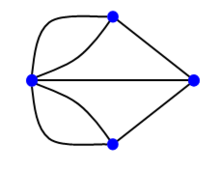
\includegraphics[width=4cm, height=4cm]{pontes}
    \caption{Pontes}
    \label{fig:my_label}
\end{figure}


O matemático considerou cada pedaço de terra como sendo um ponto, e as pontes da cidade, como sendo a ligação entre esses pontos, chamaremos eles, respectivamente, de vértices e arestas. Note que, em três dos vértices, saem três arestas de cada um, isso significa que esses vértices possuem grau três, o mesmo vale para o vértice de grau cinco, noqual saem cinco arestas. Agora, para passarmos por todas as arestas desse grafo uma única vez, precisaríamos de uma quantidade par de arestas saindo de cada vértice, pois seria necessária uma aresta de entrada e uma de saida. Assim, para o problema das pontes de Königsberg ter solução, é indispensável que o grau dos vértices seja par.

Essa contribuição de Leonard Euler foi tão significativa para a matemática, que acabou sendo o "ponta-pé inicial" de uma das áreas de estudo mais importantes da atualidade, as redes.

\section{Redes}

Uma rede é um sistema onde suas partes individuais estão ligadas de alguma maneira e, como vimos, um grafo representa essa propriedade de maneira excelente. Alguns dos explos mais famosos de redes são: a internet, onde os vértices são os computadores e as arestas poderiam ser o tráfico de dados; poderíamos descrever, também, as interações sociais, representando as pessoas como sendo os vértices e suas amizades como as arestas.



Diversos aspectos das redes são objetos de estudo hoje, porém destacaremos um dos mais importantes para entender esses sistemas, que seria o padrão das conexões entre os componentes. Imagine uma rede de interações sociais, o padrão das conexões nela existente afeta como as pessoas formam e disseminam opiniões. Com isso, podemos estudar uma das problematicas mais comuns atualmente, a disseminação de notícias falsas, popularmente conhecidas como,  \textit{fake news}. É claro que outra rede que tem grande influência nesse problema é a rede de tráfico de dados através da internet, entretanto não discutiremos essa questão a fundo. Desse modo, percebe-se a importância dos padrões encontrados nas conexões de uma rede e o que eles descrevem.
 

\end{document}
